\documentclass{article}

\usepackage[main=english,vietnamese]{babel}
\usepackage[T1]{fontenc}
\usepackage[utf8]{inputenc}
\usepackage[sexy]{evan}
\usepackage{matchsticks}
\usepackage{wrapfig}
\usepackage{listings}

\newtheorem{hint}{Hint}

\title{Test Problems fore UMC K1}
\author{Nghia Doan}
\date{\today}

\begin{document}

\maketitle

\begin{problem}[Problem One]
    Given a triangle $ABC$ satisfying $AB+BC=3\cdot AC$.
    The incircle of triangle $ABC$ has center $I$ and touches the sides $AB$ and $BC$ at the points $D$ and $E$, respectively.
    Let $K$ and $L$ be the reflections of the points $D$ and $E$ with respect to $I$.
    Let $P$ be the other intersection of $BI$ with the circumcircle $(ABC).$
    Prove that the points $A$, $C$, $K$, $L$ lie on a circle centred at $P.$
\end{problem}

\begin{proof}
    Let $M$ be the midpoint of $AC$ and $N$ the projection of $P$ to $IK.$
    Since $AB + BC = 3AC,$ we get $BD = BE = AC$, so $BD = 2CM.$

    Furthermore, $\angle ABP = \angle ACP,$ therefore $\triangle DBI$ and $\triangle MCP$ are similar in ratio $2.$
    \begin{center}
        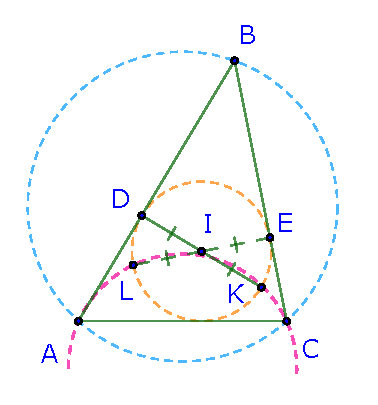
\includegraphics[width=5cm]{../Learning-Problem-Solving-2nd-Edition/png/imo-sl-2005-g1.png}
    \end{center}

    It is known that $PA = PI = PC.$
    Moreover, $\angle NPI = \angle DBI,$ so that the triangles $PNI$ and $CMP$ are congruent.
    Hence $ID = 2PM = 2IN;$ i. e. $N$ is the midpoint of $IK.$

    This shows that $PN$ is the perpendicular bisector of $IK,$ so $PC = PK = PI.$
    Analogously, $PA = PL = PI.$ So $P$ is the centre of the circle through $A, K, I, L$ and $C.$
\end{proof}

\newpage

\begin{problem}[Problem Two]
    In triangle $ABC,$ let $BC$ be the longest side. Point $X$ is chosen on side $AB$ such that $BX = BC.$
    Similarly, point $Y$ is chosen on $AC$ such that $CY = BC.$
    Prove that $OI$ is perpendicular to $XY,$ where $O$ and $I$ are the circumcenter and incenter, respectively, of triangle $ABC.$
\end{problem}

\begin{center}
    \includegraphics[width=9cm]{../Learning-Problem-Solving-2nd-Edition/svg/pdf/24-25-s7-g3-p9.pdf}
\end{center}

\newpage

\begin{proof}
    Let $AB=c, BC=a, CA=b.$ Then 

    \begin{center}
        \includegraphics[width=9cm]{../Learning-Problem-Solving-2nd-Edition/svg/pdf/24-25-s7-g3-p9-2.pdf}
    \end{center}
    
    \[ 
        \begin{aligned}
            &XA = a-c, AD=\frac{c}{2}, DX = DA + XA = \frac{c}{2} + (a-c) = a - \frac{c}{2}\\
            &OX^2 = OD^2 + DX^2 = OA^2 - AD^2 + DX^2 = OA^2 - \left(\frac{c}{2}\right)^2 + \left(a - \frac{c}{2}\right)^2 = OA^2 + a(a-c)\\
            &\text{Similarly}\ OY^2 = OA^2 + a(a-b) \Rightarrow OY^2 - OX^2 = a(c-b).
        \end{aligned}
    \]

    Similarly for $I,$
    \[ 
        \begin{aligned}
            &YA=a-b, EA = \frac{c+b-a}{2}, EY = EA + YA = \frac{c+a-b}{2}\\
            &IY^2 = IE^2 + EY^2 = IA^2 - EA^2 + EY^2 = IA^2 - \left(\frac{c+b-a}{2}\right)^2 + \left(\frac{c+a-b}{2}\right)^2 = IA^2 + c(a-b)\\
            &\text{Similarly}\ IX^2 = IA^2 + b(a-c) \Rightarrow IY^2 - IX^2 = a(c-b).
        \end{aligned}
    \]

    Hence, by the Perpendicularity Lemma $OI$ is perpendicular to $XY.$
\end{proof}

\newpage

\begin{problem}[Problem Three]
    $25$ flies are resting on the outdoor table in the garden, waiting for lunch to be served.
    \begin{itemize}[topsep=0pt, partopsep=0pt, itemsep=0pt]
        \ii It is known that for any $3$ of them, $2$ are at a distance less than $20$ cm.
        \ii There are at least a pair of flies that are further than $20$ cm from each other.
    \end{itemize}
    
    Minh's mother gave him a fly swatter, shown below, with a hoop of radius $20$ cm,
    With a single strike he can swat the flies where the hoop landed.
    In \textit{at least} how many strikes can he swat all of them?

    \textit{Assume that Minh is so fast that the flies do not have time for reaction during and between his lightning strikes.}
\end{problem}

\begin{center}
    \includegraphics[width=3.5cm]{../Learning-Problem-Solving-2nd-Edition/png/hc-2021-2-2-15.jpg}
\end{center}

\begin{soln}
    If no $2$ flies are further than $20$ cm from each other,
    Minh can strike them all in $1$ strike by aiming the center of the swatter at any fly. 
    But this is not the case, so let's assume there are $2$ flies, $A$ and $B$, that are more than $20$ cm apart.

    Then, every other fly is either in a $20$ cm radius of $A$ or in a $20$ cm radius of $B.$
    Out of the $23$ remaining flies either at least $12$ will be in the $20$ cm radius of $A$
    or $12$ will be in the $20$ cm radius of $B$.

    Swatting that the $A$ or $B$ fly with the center of the swatter kills at least $13$.
    Thus, by \framebox{$2$} strikes, he can swat them all.
\end{soln}

\end{document}